% Model 2 sketch: concise logic chain, 4 core formulas, visual restriction chart,
% and results aligned with Task 2's three questions in Problem B.
\subsection{Optimal Investment, Scheduling and Resource Allocation}\label{sec:model2}
Task~2 turns Model~1 into a 15-year dynamic decision problem: how much belt to plant each year, how to schedule ecological water and labour, and how to split funds among construction, O\&M and photovoltaics (PV) under a fixed budget.

Planting and PV installation create dated cohorts. The optimiser carries each cohort's cover and stored water forward and charges it for water, labour and maintenance. PV competes for the construction budget and subsequently earns revenue (Figure~\ref{fig:m2-struct}).

\begin{figure}[!htb]
  \centering
  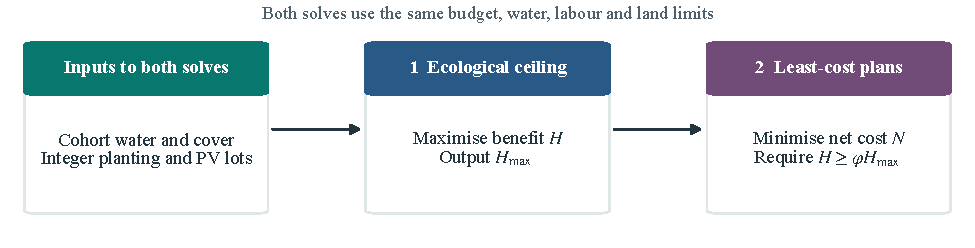
\includegraphics[width=\linewidth]{../Figures/Paper2026_Polished/fig09_two_stage_optimisation.pdf}
  \caption{Two-stage optimisation of the planting and PV plan.}
  \label{fig:m2-struct}
\end{figure}

\subsubsection[Cohort Irrigation, PV Revenue, and Resource Limits]{Model construction}
\paragraph{Cohort formulation and ecological benefit.} Tracking only total area $A_t$ cannot distinguish a newly planted shrub ($V_0=2\%$, low water demand) from an older stand ($>12\%$ cover, high summer demand). Instead, we bind each planting year $s\in\{1,\dots,T\}$ and lifetime watering recipe $p\in\mathcal P$ into a \textbf{cohort block} $(s,p)$ ($18$ recipes: constant $0\text{--}1{,}000$\,mm/yr, step-up or step-down after age $3$ or $5$, and a $100\to300\to600$\,mm/yr ramp). Because field engineering is deployed in discrete lots rather than arbitrary square metres, belt area and PV capacity are added in integer multiples of minimum step thresholds $\Delta_A$ and $\Delta_P$: $a_{s,p}=\Delta_A n_{s,p}$ and $y_s=\Delta_P z_s$, giving active belt stock $A_t=\sum_{s\le t,p}a_{s,p}$, installed PV $P_t^{\mathrm{inst}}=\sum_{s\le t}y_s$, and operating PV $P_t^{\mathrm{op}}=\sum_{s<t}y_s$ (panels built in year $s$ generate from year $s+1$).



Each cohort runs Model~1's daily water bucket $\mathcal W$ (Algorithm~\ref{alg:m1}) under its age-specific quota $q_{p,t-s}$ and updates cover via Eq.~\eqref{eq:m1-veg}. Summing start-of-year cover relative to the local ceiling $K$ across all active cohorts defines the 15-year ecological benefit:
\begin{equation}\label{eq:m2-eco}
H=\sum_{t=1}^{T}\sum_{s\le t,\,p\in\mathcal P}\underbrace{a_{s,p}\,\frac{V_{s,p,t}}{K}}_{\text{effective ha in year }t},\qquad
(M_{s,p,t+1},\,\overline W_{s,p,t})=\mathcal W\!\big(V_{s,p,t},\,M_{s,p,t},\,q_{p,t-s}\big).
\end{equation}
One hectare at $V=K$ for one year scores $1\text{ effective ha}\cdot\text{yr}$. Using start-of-year cover $V_{s,p,t}$ avoids crediting growth before it happens and naturally rewards early planting because desert shrubs take a decade to mature.

\paragraph{Investment allocation ratios and PV revenue.} In year $t$, gross spending $D_t$ splits across Task~2's three required uses---construction, O\&M (including water delivery $Q_t$), and PV capital---while operating panels earn electricity revenue $R_t$:
\begin{equation}\label{eq:m2-cash}
D_t=\underbrace{c_b a_t}_{C_t^b:\ \text{build}}+\underbrace{\big(c_m A_t+c_{pm}P_t^{\mathrm{op}}+c_w Q_t\big)}_{C_t^o:\ \text{O\&M + water}}+\underbrace{c_p y_t}_{C_t^p:\ \text{PV}},\quad
R_t=p_e\!\sum_{s<t}y_s e_0(1-d_p)^{t-s-1}.
\end{equation}
Here $a_t=\sum_p a_{t,p}$ is newly treated area, $(f_t^b,f_t^o,f_t^p)=(C_t^b,C_t^o,C_t^p)/D_t$ ($f_t^b+f_t^o+f_t^p=1$ when $D_t>0$) is the annual \textbf{investment allocation ratio}, $e_0$ is first-year net grid yield per kW, $d_p=0.5\%/\text{yr}$ is panel degradation \cite{EN06}, and $p_e$ is the scenario settlement tariff (Table~\ref{tab:m2-par}).

\paragraph{Resource constraints and ecological target.} Table~\ref{tab:m2-caps} specifies the limits on new construction and ongoing operations. Capital is paid at the start of year $t$, and operating costs and revenue are recorded at year-end, with real discount factor $\delta=(1+i_d)^{-1}$. We use a two-step $\varepsilon$-constraint formulation to balance ecological benefit and cost:
\begin{equation}\label{eq:m2-eps}
\min_{\bm n,\bm z}\ N=\sum_{t=1}^{T}\Big[\underbrace{\delta^{t-1}\big(C_t^b+C_t^p\big)}_{\text{year-start capex}}+\underbrace{\delta^{t}\big(C_t^o-R_t\big)}_{\text{year-end O\&M $-$ PV}}\Big]
\;\;\text{s.t.}\;\; H\ge\varphi H_{\max},\ \text{Table~\ref{tab:m2-caps} limits},
\end{equation}
where Step~1 maximises $H$ under the same caps to find the physical ceiling $H_{\max}$, and Step~2 minimises net present cost $N$ for a chosen ecological target share $\varphi\in[0,1]$ ($\varphi=0.60$ in the baseline).

\begin{table}[H]
  \centering
  \caption{Baseline resource constraints for the 15-year plan.}
  \label{tab:m2-caps}
  \small
  \renewcommand{\arraystretch}{1.08}
  \begin{tabularx}{\linewidth}{@{}l >{\raggedright\arraybackslash}X >{\raggedright\arraybackslash}p{0.34\linewidth}@{}}
    \toprule
    \textbf{Resource} & \textbf{Quantity constrained} & \textbf{Baseline limit} \\
    \midrule
    Funding & Gross spending on planting, PV, and upkeep, including water &
      $D_t\le 12$ million CNY per year\newline
      $\sum_t D_t\le 80$ million CNY in total \\
    \addlinespace[2pt]
    Water & Irrigation for every active cohort plus washing for operating PV &
      $Q_t\le 1.50$ million m$^3$ per year\newline
      $Q_{t,m}\le$ monthly canal cap (30{,}000--240{,}000 m$^3$) \\
    \addlinespace[2pt]
    Land & Active shelterbelt plus installed PV footprint ($\alpha_p=0.002$\,ha/kW) &
      $A_t+\alpha_p P_t^{\mathrm{inst}}\le 1{,}200$\,ha \\
    Construction & Newly planted shelterbelt area & $a_t\le 200$\,ha per year \\
    Grid & Cumulative installed PV capacity & $P_t^{\mathrm{inst}}\le 10$\,MW \\
    \addlinespace[2pt]
    Labour & New planting and PV installation plus upkeep of the belt and operating PV &
      $L_t\le 12{,}000$ person-days per year \\
    \bottomrule
  \end{tabularx}
\end{table}

\subsubsection[Two-Step MILP for Ecological Targets and Cost]{Solution approach}
Pre-simulating the 18 schedules in Model~1 converts Eq.~\eqref{eq:m2-eps} into an exact mixed-integer linear programme (MILP) over integer block counts $\bm x=(\bm n,\bm z)$, solved via branch-and-cut (HiGHS, MIP gap tolerance $0.20\%$; Algorithm~\ref{alg:m2-milp}). Every solved plan is independently replayed forward through Model~1 to verify water and cash closure (maximum discrepancy $1.9\times10^{-9}$). Because the problem statement gives no site budget, water quota or tariff, Table~\ref{tab:m2-par} sets an auditable 15-year planning scenario anchored to a 2024 Yutian desert-treatment trial ($52{,}500$\,CNY/ha \cite{REF20}) and literature PV degradation \cite{EN06}.

\begin{algorithm}[!htb]
\caption{Cohort pre-simulation and two-step $\varepsilon$-constraint MILP}\label{alg:m2-milp}
\begin{algorithmic}[1]
\Require Model~1 $(r,d,K,\mathcal W)$, 18-policy library $\mathcal P$, scenario parameters and limits (Tables~\ref{tab:m2-caps} and \ref{tab:m2-par})
\Ensure optimal schedule $\bm x^*$, ceiling $H_{\max}$, trade-off points and sensitivity runs
\State Run Model~1 (Algorithm~\ref{alg:m1}) once per policy $p\in\mathcal P$ from $(V_0,M_0)$ to tabulate per-ha $V_{\mathrm{start}}$ and monthly water
\State Build linear constraint matrix $\bm A\bm x\le\bm b$, ecology vector $\bm h$ (Eq.~\eqref{eq:m2-eco}) and net cost vector $\bm c$ (Eq.~\eqref{eq:m2-eps})
\State \textbf{Step 1:} $H_{\max}\gets\max\{\bm h^\top\bm x:\bm A\bm x\le\bm b,\ \bm x\in\mathbb Z_{\ge0}^m\}$;\quad \textbf{Step 2:} $\bm x^*\gets\arg\min\{\bm c^\top\bm x:\bm A\bm x\le\bm b,\ \bm h^\top\bm x\ge\varphi H_{\max}\}$
\State Sweep $\varphi\in\{0,0.2,\dots,1.0\}$; perturb parameters at fixed $H\ge0.60\,H_{\max}$; replay chosen cohorts in Model~1
\end{algorithmic}
\end{algorithm}

\begin{table}[H]
\centering\small
\caption{Model~2 scenario parameters and sensitivity ranges.}
\label{tab:m2-par}
\renewcommand{\arraystretch}{1.06}
\begin{tabularx}{\linewidth}{@{}l X r c l@{}}
\toprule
Symbol & Meaning & Base value & Tested / note & Unit \\
\midrule
$T;\ \Delta_A,\Delta_P$ & horizon; min.\ lot thresholds ($\Delta_A=25$\,ha tested; $V_0=2\%$) & $15;\ 50,\ 100$ & $V_0$: 1--4\% & yr; ha, kW \\
$c_b,\ c_m,\ c_w$ & planting capex \cite{REF20}, belt O\&M, water unit cost & $52{,}500,\ 1{,}500,\ 1.0$ & $c_b\pm25\%$, $c_m\pm50\%$ & CNY (ha, m$^3$) \\
$c_p,\ c_{pm}$ & PV turnkey capex and annual O\&M rate & $3{,}000,\ 50$ & $c_p\pm25\%$ & CNY/kW \\
$e_0,\ p_e,\ d_p$ & 1st-yr PV yield, tariff, degradation \cite{EN06} ($w_c=0.02$\,m$^3$/kW) & $1{,}500,\ 0.30,\ 0.5\%$ & $p_e$: 0.15--0.40 & kWh, CNY, /yr \\
$\ell_b,\ell_m;\ \ell_p,\ell_{pm}$ & belt build/O\&M and PV build/O\&M labour rates & $30,3;\ 0.10,0.01$ & turnkey wages & p-d / (ha, kW) \\
$i_d;\ \varphi$ & real discount rate; baseline ecological target share & $5\%;\ 60\%$ & $\varphi$: 0--100\% & -- \\
\bottomrule
\end{tabularx}
\end{table}

\subsubsection[15-Year Plan and Effects of Tariffs and Seedling Cover]{Results}
\paragraph{Optimal 15-year trajectory.} The ecological maximum is $H_{\max}=2{,}097$ effective hectare-years. It uses $900$\,ha and no PV, at a net present cost of $64.4$\,M\,CNY. The least-cost plan at the $60\%$ target costs $25.35$\,M\,CNY and delivers $1{,}265$ effective hectare-years. Figure~\ref{fig:m2-plan} shows when the plan invests and how the planted cohorts enter Model~3.
\begin{enumerate}\setlength{\itemsep}{2pt}\setlength{\parsep}{0pt}
  \item \textbf{Newly treated area.} Plant $150$\,ha in each of the first two years, for $300$\,ha in total. Early planting gives stands more years to accumulate ecological benefit.
  \item \textbf{Water replenishment.} At low cover, the model gives young stands a low transpiration demand. The selected schedules use $100$\,mm/yr for the first three years, then $300$\,mm/yr at age~4. The $50$\,ha core strip rises to $600$\,mm/yr at age~8 (Figure~\ref{fig:m2-plan}a). From project year~8, annual use is about $70\%$ of its cap and May use reaches $95\%$ of the monthly cap (Figure~\ref{fig:m2-water}).
  \item \textbf{Investment allocation.} Build $9.5$\,MW of PV in years 1--4. Planting takes $66\%$ of year-1 spending, PV takes about $90\%$ in years 3--4, and O\&M accounts for all spending from year~5 (Figure~\ref{fig:m2-plan}b). Electricity income of $4.1\text{--}4.3$\,M\,CNY/yr offsets annual O\&M and water expenditures of $1.8\text{--}2.0$\,M\,CNY after year~4. Net present cost is about $9\%$ below the best PV-free plan.
  \item \textbf{Labour input.} Demand peaks at $5{,}522$ person-days in year~2 and settles at $995$ person-days/yr from year~5, within the $12{,}000$ person-day cap.
\end{enumerate}

\begin{figure}[!htb]
  \centering
  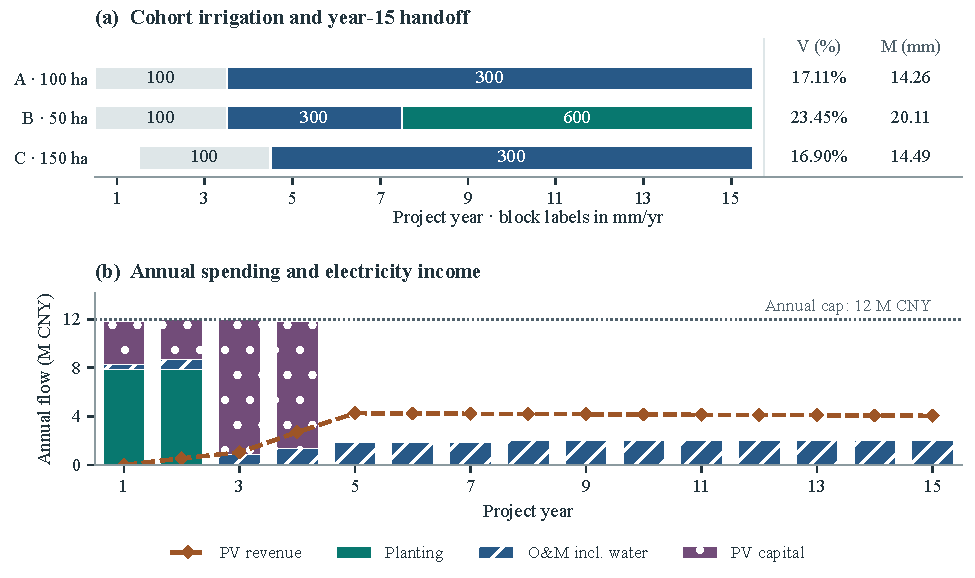
\includegraphics[width=\linewidth]{../Figures/Paper2026_Polished/fig10_cohort_plan.pdf}
  \caption{Cohort irrigation, final states and annual cash flows at the 60\% target.}
  \label{fig:m2-plan}
\end{figure}

\begin{figure}[!htbp]
  \centering
  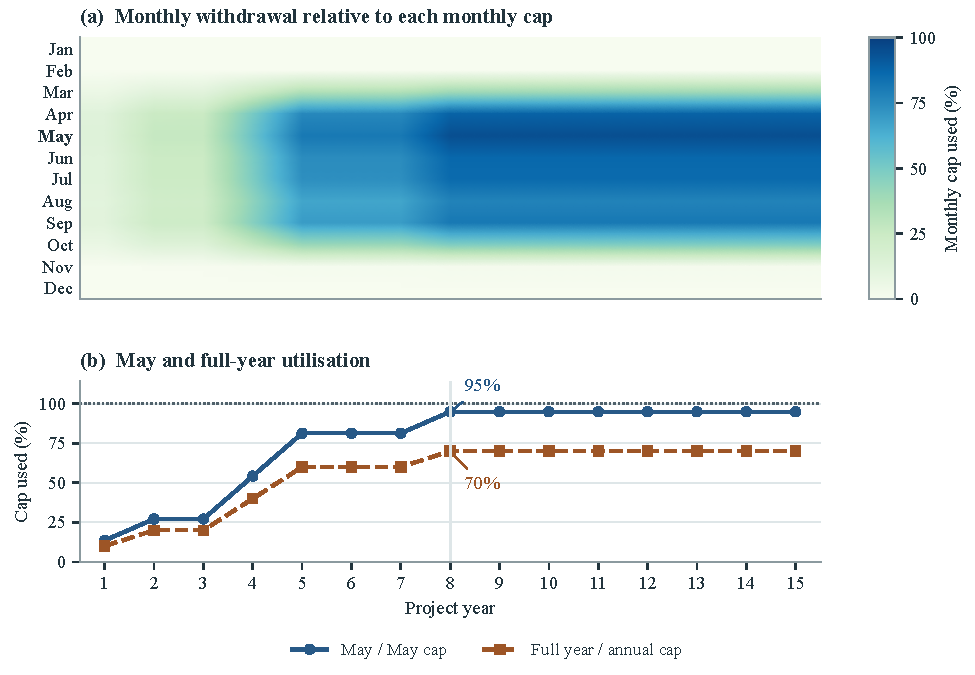
\includegraphics[width=\linewidth]{../Figures/Paper2026_Polished/fig11_water_use_smooth.pdf}
  \caption{Monthly withdrawals and the May bottleneck (interpolated shading).}
  \label{fig:m2-water}
\end{figure}

\paragraph{Balancing ecology against cost.} Up to the $60\%$ target, net present cost rises by $23\text{--}26$\,k\,CNY per added effective hectare-year across the solved targets. This increment rises to $36.7$\,k from $60\%$ to $80\%$ and $57.1$\,k from $80\%$ to $100\%$, as PV falls from $9.5$ to $5.3$\,MW and then to zero (Figure~\ref{fig:m2-tradeoff}).

For a candidate build year, the standalone tariff screen divides discounted cost by discounted generation through year~15, excluding resource opportunity costs, tax and financing. The tariff of $0.30$\,CNY/kWh clears the year-4 requirement of $0.293$ but falls short of $0.312$ in year~5. The MILP then accounts for scarce water, labour and capital.

\begin{figure}[!htbp]
  \centering
  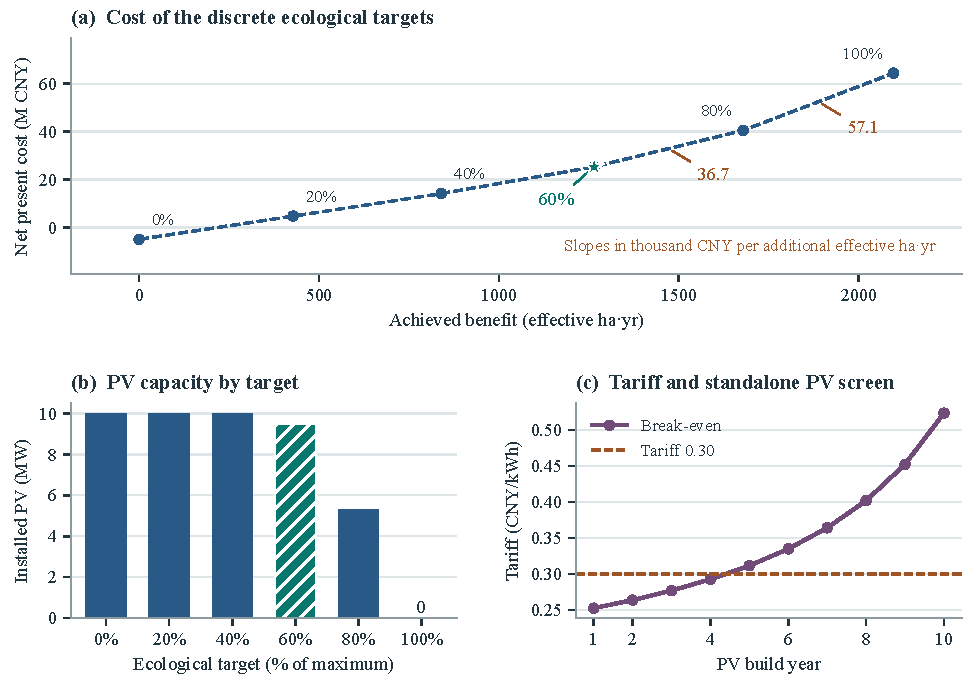
\includegraphics[width=\linewidth]{../Figures/Paper2026_Polished/fig12_tradeoff.pdf}
  \caption{Cost, ecological benefit and PV viability across six targets.}
  \label{fig:m2-tradeoff}
\end{figure}

\paragraph{Investment sensitivity.} At the same absolute ecological target, restricting the policy library to constant irrigation raises net present cost from $25.35$ to $27.04$\,M\,CNY, or about $6.6\%$ relative to the baseline. A tariff of $0.15$\,CNY/kWh or PV capex of $3{,}750$\,CNY/kW eliminates PV in the corresponding plan. Raising O\&M rates by $50\%$ trims PV to $5.6$\,MW. Halving initial cover from $2\%$ to $1\%$ raises the area required to $400$\,ha and produces the largest cost increase among the cases shown (Figure~\ref{fig:m2-investment}).

\begin{figure}[!htbp]
  \centering
  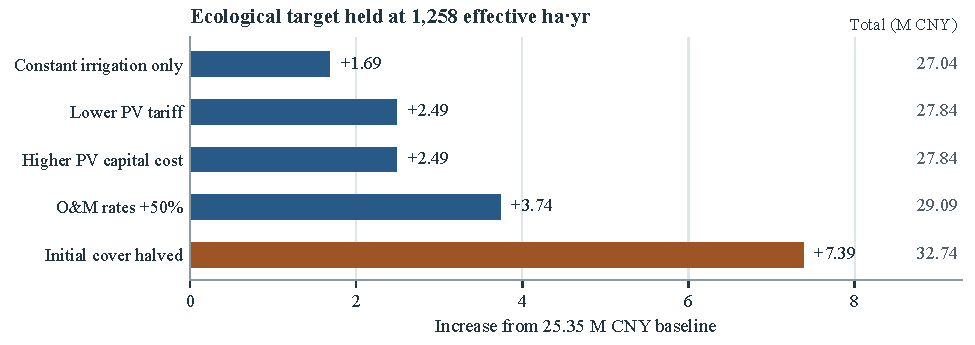
\includegraphics[width=\linewidth]{../Figures/Paper2026_Polished/fig13_investment_sensitivity.pdf}
  \caption{Cost sensitivity at a fixed ecological target.}
  \label{fig:m2-investment}
\end{figure}

\paragraph{Summary.} The conditional plan prioritizes early planting, staged irrigation and viable PV investment. May delivery capacity and seedling establishment are the main constraints to verify before adopting the plan. The completed cohorts then enter Model~3.
\FloatBarrier
